\documentclass[1p]{elsarticle_modified}
%\bibliographystyle{elsarticle-num}

%\usepackage[colorlinks]{hyperref}
%\usepackage{abbrmath_seonhwa} %\Abb, \Ascr, \Acal ,\Abf, \Afrak
\usepackage{amsfonts}
\usepackage{amssymb}
\usepackage{amsmath}
\usepackage{amsthm}
\usepackage{scalefnt}
\usepackage{amsbsy}
\usepackage{kotex}
\usepackage{caption}
\usepackage{subfig}
\usepackage{color}
\usepackage{graphicx}
\usepackage{xcolor} %% white, black, red, green, blue, cyan, magenta, yellow
\usepackage{float}
\usepackage{setspace}
\usepackage{hyperref}

\usepackage{tikz}
\usetikzlibrary{arrows}

\usepackage{multirow}
\usepackage{array} % fixed length table
\usepackage{hhline}

%%%%%%%%%%%%%%%%%%%%%
\makeatletter
\renewcommand*\env@matrix[1][\arraystretch]{%
	\edef\arraystretch{#1}%
	\hskip -\arraycolsep
	\let\@ifnextchar\new@ifnextchar
	\array{*\c@MaxMatrixCols c}}
\makeatother %https://tex.stackexchange.com/questions/14071/how-can-i-increase-the-line-spacing-in-a-matrix
%%%%%%%%%%%%%%%

\usepackage[normalem]{ulem}

\newcommand{\msout}[1]{\ifmmode\text{\sout{\ensuremath{#1}}}\else\sout{#1}\fi}
%SOURCE: \msout is \stkout macro in https://tex.stackexchange.com/questions/20609/strikeout-in-math-mode

\newcommand{\cancel}[1]{
	\ifmmode
	{\color{red}\msout{#1}}
	\else
	{\color{red}\sout{#1}}
	\fi
}

\newcommand{\add}[1]{
	{\color{blue}\uwave{#1}}
}

\newcommand{\replace}[2]{
	\ifmmode
	{\color{red}\msout{#1}}{\color{blue}\uwave{#2}}
	\else
	{\color{red}\sout{#1}}{\color{blue}\uwave{#2}}
	\fi
}

\newcommand{\Sol}{\mathcal{S}} %segment
\newcommand{\D}{D} %diagram
\newcommand{\A}{\mathcal{A}} %arc


%%%%%%%%%%%%%%%%%%%%%%%%%%%%%5 test

\def\sl{\operatorname{\textup{SL}}(2,\Cbb)}
\def\psl{\operatorname{\textup{PSL}}(2,\Cbb)}
\def\quan{\mkern 1mu \triangleright \mkern 1mu}

\theoremstyle{definition}
\newtheorem{thm}{Theorem}[section]
\newtheorem{prop}[thm]{Proposition}
\newtheorem{lem}[thm]{Lemma}
\newtheorem{ques}[thm]{Question}
\newtheorem{cor}[thm]{Corollary}
\newtheorem{defn}[thm]{Definition}
\newtheorem{exam}[thm]{Example}
\newtheorem{rmk}[thm]{Remark}
\newtheorem{alg}[thm]{Algorithm}

\newcommand{\I}{\sqrt{-1}}
\begin{document}

%\begin{frontmatter}
%
%\title{Boundary parabolic representations of knots up to 8 crossings}
%
%%% Group authors per affiliation:
%\author{Yunhi Cho} 
%\address{Department of Mathematics, University of Seoul, Seoul, Korea}
%\ead{yhcho@uos.ac.kr}
%
%
%\author{Seonhwa Kim} %\fnref{s_kim}}
%\address{Center for Geometry and Physics, Institute for Basic Science, Pohang, 37673, Korea}
%\ead{ryeona17@ibs.re.kr}
%
%\author{Hyuk Kim}
%\address{Department of Mathematical Sciences, Seoul National University, Seoul 08826, Korea}
%\ead{hyukkim@snu.ac.kr}
%
%\author{Seokbeom Yoon}
%\address{Department of Mathematical Sciences, Seoul National University, Seoul, 08826,  Korea}
%\ead{sbyoon15@snu.ac.kr}
%
%\begin{abstract}
%We find all boundary parabolic representation of knots up to 8 crossings.
%
%\end{abstract}
%\begin{keyword}
%    \MSC[2010] 57M25 
%\end{keyword}
%
%\end{frontmatter}

%\linenumbers
%\tableofcontents
%
\newcommand\colored[1]{\textcolor{white}{\rule[-0.35ex]{0.8em}{1.4ex}}\kern-0.8em\color{red} #1}%
%\newcommand\colored[1]{\textcolor{white}{ #1}\kern-2.17ex	\textcolor{white}{ #1}\kern-1.81ex	\textcolor{white}{ #1}\kern-2.15ex\color{red}#1	}

{\Large $\underline{12a_{0303}~(K12a_{0303})}$}

\setlength{\tabcolsep}{10pt}
\renewcommand{\arraystretch}{1.6}
\vspace{1cm}\begin{tabular}{m{100pt}>{\centering\arraybackslash}m{274pt}}
\multirow{5}{120pt}{
	\centering
	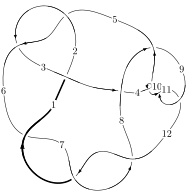
\includegraphics[width=112pt]{../../../GIT/diagram.site/Diagrams/png/1104_12a_0303.png}\\
\ \ \ A knot diagram\footnotemark}&
\allowdisplaybreaks
\textbf{Linearized knot diagam} \\
\cline{2-2}
 &
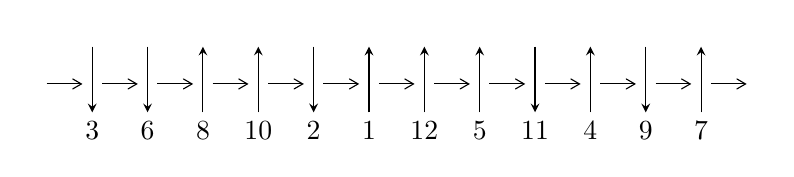
\begin{tikzpicture}[x=20pt, y=17pt]
	% nodes
	\node (C0) at (0, 0) {};
	\node (C1) at (1, 0) {};
	\node (C1U) at (1, +1) {};
	\node (C1D) at (1, -1) {3};

	\node (C2) at (2, 0) {};
	\node (C2U) at (2, +1) {};
	\node (C2D) at (2, -1) {6};

	\node (C3) at (3, 0) {};
	\node (C3U) at (3, +1) {};
	\node (C3D) at (3, -1) {8};

	\node (C4) at (4, 0) {};
	\node (C4U) at (4, +1) {};
	\node (C4D) at (4, -1) {10};

	\node (C5) at (5, 0) {};
	\node (C5U) at (5, +1) {};
	\node (C5D) at (5, -1) {2};

	\node (C6) at (6, 0) {};
	\node (C6U) at (6, +1) {};
	\node (C6D) at (6, -1) {1};

	\node (C7) at (7, 0) {};
	\node (C7U) at (7, +1) {};
	\node (C7D) at (7, -1) {12};

	\node (C8) at (8, 0) {};
	\node (C8U) at (8, +1) {};
	\node (C8D) at (8, -1) {5};

	\node (C9) at (9, 0) {};
	\node (C9U) at (9, +1) {};
	\node (C9D) at (9, -1) {11};

	\node (C10) at (10, 0) {};
	\node (C10U) at (10, +1) {};
	\node (C10D) at (10, -1) {4};

	\node (C11) at (11, 0) {};
	\node (C11U) at (11, +1) {};
	\node (C11D) at (11, -1) {9};

	\node (C12) at (12, 0) {};
	\node (C12U) at (12, +1) {};
	\node (C12D) at (12, -1) {7};
	\node (C13) at (13, 0) {};

	% arrows
	\draw[->,>={angle 60}]
	(C0) edge (C1) (C1) edge (C2) (C2) edge (C3) (C3) edge (C4) (C4) edge (C5) (C5) edge (C6) (C6) edge (C7) (C7) edge (C8) (C8) edge (C9) (C9) edge (C10) (C10) edge (C11) (C11) edge (C12) (C12) edge (C13) ;	\draw[->,>=stealth]
	(C1U) edge (C1D) (C2U) edge (C2D) (C3D) edge (C3U) (C4D) edge (C4U) (C5U) edge (C5D) (C6D) edge (C6U) (C7D) edge (C7U) (C8D) edge (C8U) (C9U) edge (C9D) (C10D) edge (C10U) (C11U) edge (C11D) (C12D) edge (C12U) ;
	\end{tikzpicture} \\
\hhline{~~} \\& 
\textbf{Solving Sequence} \\ \cline{2-2} 
 &
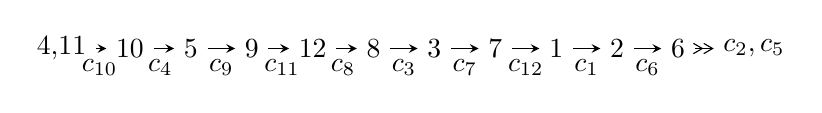
\begin{tikzpicture}[x=22pt, y=7pt]
	% node
	\node (A0) at (-1/8, 0) {4,11};
	\node (A1) at (1, 0) {10};
	\node (A2) at (2, 0) {5};
	\node (A3) at (3, 0) {9};
	\node (A4) at (4, 0) {12};
	\node (A5) at (5, 0) {8};
	\node (A6) at (6, 0) {3};
	\node (A7) at (7, 0) {7};
	\node (A8) at (8, 0) {1};
	\node (A9) at (9, 0) {2};
	\node (A10) at (10, 0) {6};
	\node (C1) at (1/2, -1) {$c_{10}$};
	\node (C2) at (3/2, -1) {$c_{4}$};
	\node (C3) at (5/2, -1) {$c_{9}$};
	\node (C4) at (7/2, -1) {$c_{11}$};
	\node (C5) at (9/2, -1) {$c_{8}$};
	\node (C6) at (11/2, -1) {$c_{3}$};
	\node (C7) at (13/2, -1) {$c_{7}$};
	\node (C8) at (15/2, -1) {$c_{12}$};
	\node (C9) at (17/2, -1) {$c_{1}$};
	\node (C10) at (19/2, -1) {$c_{6}$};
	\node (A11) at (45/4, 0) {$c_{2},c_{5}$};

	% edge
	\draw[->,>=stealth]	
	(A0) edge (A1) (A1) edge (A2) (A2) edge (A3) (A3) edge (A4) (A4) edge (A5) (A5) edge (A6) (A6) edge (A7) (A7) edge (A8) (A8) edge (A9) (A9) edge (A10) ;
	\draw[->>,>={angle 60}]	
	(A10) edge (A11);
\end{tikzpicture} \\ 

\end{tabular} \\

\footnotetext{
The image of knot diagram is generated by the software ``\textbf{Draw programme}" developed by Andrew Bartholomew(\url{http://www.layer8.co.uk/maths/draw/index.htm\#Running-draw}), where we modified some parts for our purpose(\url{https://github.com/CATsTAILs/LinksPainter}).
}\phantom \\ \newline 
\centering \textbf{Ideals for irreducible components\footnotemark of $X_{\text{par}}$} 
 
\begin{align*}
I^u_{1}&=\langle 
u^{76}+u^{75}+\cdots- u^2+1\rangle \\
\\
\end{align*}
\raggedright * 1 irreducible components of $\dim_{\mathbb{C}}=0$, with total 76 representations.\\
\footnotetext{All coefficients of polynomials are rational numbers. But the coefficients are sometimes approximated in decimal forms when there is not enough margin.}
\newpage
\renewcommand{\arraystretch}{1}
\centering \section*{I. $I^u_{1}= \langle u^{76}+u^{75}+\cdots- u^2+1 \rangle$}
\flushleft \textbf{(i) Arc colorings}\\
\begin{tabular}{m{7pt} m{180pt} m{7pt} m{180pt} }
\flushright $a_{4}=$&$\begin{pmatrix}0\\u\end{pmatrix}$ \\
\flushright $a_{11}=$&$\begin{pmatrix}1\\0\end{pmatrix}$ \\
\flushright $a_{10}=$&$\begin{pmatrix}1\\u^2\end{pmatrix}$ \\
\flushright $a_{5}=$&$\begin{pmatrix}u\\u^3+u\end{pmatrix}$ \\
\flushright $a_{9}=$&$\begin{pmatrix}u^2+1\\u^2\end{pmatrix}$ \\
\flushright $a_{12}=$&$\begin{pmatrix}u^4+u^2+1\\u^4\end{pmatrix}$ \\
\flushright $a_{8}=$&$\begin{pmatrix}u^6+u^4+2 u^2+1\\u^8+2 u^6+2 u^4+2 u^2\end{pmatrix}$ \\
\flushright $a_{3}=$&$\begin{pmatrix}- u^{13}-2 u^{11}-5 u^9-6 u^7-6 u^5-4 u^3- u\\- u^{15}-3 u^{13}-6 u^{11}-9 u^9-8 u^7-6 u^5-2 u^3+u\end{pmatrix}$ \\
\flushright $a_{7}=$&$\begin{pmatrix}- u^{16}-3 u^{14}-7 u^{12}-10 u^{10}-11 u^8-8 u^6-4 u^4+1\\- u^{16}-2 u^{14}-4 u^{12}-4 u^{10}-2 u^8+2 u^4+2 u^2\end{pmatrix}$ \\
\flushright $a_{1}=$&$\begin{pmatrix}u^{28}+5 u^{26}+\cdots- u^2+1\\u^{28}+4 u^{26}+\cdots-10 u^6-3 u^4\end{pmatrix}$ \\
\flushright $a_{2}=$&$\begin{pmatrix}u^{56}+9 u^{54}+\cdots-2 u^2+1\\u^{58}+10 u^{56}+\cdots-8 u^4+u^2\end{pmatrix}$ \\
\flushright $a_{6}=$&$\begin{pmatrix}- u^{40}-7 u^{38}+\cdots-2 u^2+1\\- u^{40}-6 u^{38}+\cdots+2 u^4+2 u^2\end{pmatrix}$\\&\end{tabular}
\flushleft \textbf{(ii) Obstruction class $= -1$}\\~\\
\flushleft \textbf{(iii) Cusp Shapes $= -4 u^{74}-4 u^{73}+\cdots+8 u+2$}\\~\\
\newpage\renewcommand{\arraystretch}{1}
\flushleft \textbf{(iv) u-Polynomials at the component}\newline \\
\begin{tabular}{m{50pt}|m{274pt}}
Crossings & \hspace{64pt}u-Polynomials at each crossing \\
\hline $$\begin{aligned}c_{1}\end{aligned}$$&$\begin{aligned}
&u^{76}+43 u^{75}+\cdots+2 u+1
\end{aligned}$\\
\hline $$\begin{aligned}c_{2},c_{5}\end{aligned}$$&$\begin{aligned}
&u^{76}+u^{75}+\cdots+2 u+1
\end{aligned}$\\
\hline $$\begin{aligned}c_{3}\end{aligned}$$&$\begin{aligned}
&u^{76}+u^{75}+\cdots+4 u+1
\end{aligned}$\\
\hline $$\begin{aligned}c_{4},c_{10}\end{aligned}$$&$\begin{aligned}
&u^{76}+u^{75}+\cdots- u^2+1
\end{aligned}$\\
\hline $$\begin{aligned}c_{6},c_{7},c_{12}\end{aligned}$$&$\begin{aligned}
&u^{76}+3 u^{75}+\cdots+85 u+16
\end{aligned}$\\
\hline $$\begin{aligned}c_{8}\end{aligned}$$&$\begin{aligned}
&u^{76}-5 u^{75}+\cdots-374 u+31
\end{aligned}$\\
\hline $$\begin{aligned}c_{9},c_{11}\end{aligned}$$&$\begin{aligned}
&u^{76}+25 u^{75}+\cdots-2 u+1
\end{aligned}$\\
\hline
\end{tabular}\\~\\
\newpage\renewcommand{\arraystretch}{1}
\flushleft \textbf{(v) Riley Polynomials at the component}\newline \\
\begin{tabular}{m{50pt}|m{274pt}}
Crossings & \hspace{64pt}Riley Polynomials at each crossing \\
\hline $$\begin{aligned}c_{1}\end{aligned}$$&$\begin{aligned}
&y^{76}-19 y^{75}+\cdots+6 y+1
\end{aligned}$\\
\hline $$\begin{aligned}c_{2},c_{5}\end{aligned}$$&$\begin{aligned}
&y^{76}-43 y^{75}+\cdots-2 y+1
\end{aligned}$\\
\hline $$\begin{aligned}c_{3}\end{aligned}$$&$\begin{aligned}
&y^{76}+y^{75}+\cdots+270 y+1
\end{aligned}$\\
\hline $$\begin{aligned}c_{4},c_{10}\end{aligned}$$&$\begin{aligned}
&y^{76}+25 y^{75}+\cdots-2 y+1
\end{aligned}$\\
\hline $$\begin{aligned}c_{6},c_{7},c_{12}\end{aligned}$$&$\begin{aligned}
&y^{76}+81 y^{75}+\cdots+13735 y+256
\end{aligned}$\\
\hline $$\begin{aligned}c_{8}\end{aligned}$$&$\begin{aligned}
&y^{76}+13 y^{75}+\cdots-24866 y+961
\end{aligned}$\\
\hline $$\begin{aligned}c_{9},c_{11}\end{aligned}$$&$\begin{aligned}
&y^{76}+53 y^{75}+\cdots-10 y+1
\end{aligned}$\\
\hline
\end{tabular}\\~\\
\newpage\flushleft \textbf{(vi) Complex Volumes and Cusp Shapes}
$$\begin{array}{c|c|c}  
\text{Solutions to }I^u_{1}& \I (\text{vol} + \sqrt{-1}CS) & \text{Cusp shape}\\
 \hline 
\begin{aligned}
u &= -0.549992 + 0.839426 I\end{aligned}
 & -1.86851 + 0.80066 I & \phantom{-0.000000 } 0 \\ \hline\begin{aligned}
u &= -0.549992 - 0.839426 I\end{aligned}
 & -1.86851 - 0.80066 I & \phantom{-0.000000 } 0 \\ \hline\begin{aligned}
u &= \phantom{-}0.734078 + 0.689064 I\end{aligned}
 & -0.233189 - 0.030227 I & \phantom{-0.000000 } 0 \\ \hline\begin{aligned}
u &= \phantom{-}0.734078 - 0.689064 I\end{aligned}
 & -0.233189 + 0.030227 I & \phantom{-0.000000 } 0 \\ \hline\begin{aligned}
u &= -0.128262 + 1.010270 I\end{aligned}
 & -3.91459 - 5.98588 I & \phantom{-0.000000 -}0. + 8.65263 I \\ \hline\begin{aligned}
u &= -0.128262 - 1.010270 I\end{aligned}
 & -3.91459 + 5.98588 I & \phantom{-0.000000 } 0. - 8.65263 I \\ \hline\begin{aligned}
u &= -0.053301 + 1.017620 I\end{aligned}
 & -5.69296 + 0.01431 I & -9.46209 + 0. I\phantom{ +0.000000I} \\ \hline\begin{aligned}
u &= -0.053301 - 1.017620 I\end{aligned}
 & -5.69296 - 0.01431 I & -9.46209 + 0. I\phantom{ +0.000000I} \\ \hline\begin{aligned}
u &= \phantom{-}0.105691 + 0.972796 I\end{aligned}
 & -2.05395 + 2.01148 I & \phantom{-0.000000 } 0. - 4.13806 I \\ \hline\begin{aligned}
u &= \phantom{-}0.105691 - 0.972796 I\end{aligned}
 & -2.05395 - 2.01148 I & \phantom{-0.000000 -}0. + 4.13806 I \\ \hline\begin{aligned}
u &= -0.803027 + 0.656543 I\end{aligned}
 & -6.37926 + 0.22483 I & \phantom{-0.000000 } 0 \\ \hline\begin{aligned}
u &= -0.803027 - 0.656543 I\end{aligned}
 & -6.37926 - 0.22483 I & \phantom{-0.000000 } 0 \\ \hline\begin{aligned}
u &= \phantom{-}0.805471 + 0.664918 I\end{aligned}
 & -2.39312 - 4.72743 I & \phantom{-0.000000 } 0 \\ \hline\begin{aligned}
u &= \phantom{-}0.805471 - 0.664918 I\end{aligned}
 & -2.39312 + 4.72743 I & \phantom{-0.000000 } 0 \\ \hline\begin{aligned}
u &= -0.812427 + 0.664787 I\end{aligned}
 & -5.89683 + 9.60757 I & \phantom{-0.000000 } 0 \\ \hline\begin{aligned}
u &= -0.812427 - 0.664787 I\end{aligned}
 & -5.89683 - 9.60757 I & \phantom{-0.000000 } 0 \\ \hline\begin{aligned}
u &= -0.777148 + 0.718369 I\end{aligned}
 & \phantom{-}3.81626 + 1.47965 I & \phantom{-0.000000 } 0 \\ \hline\begin{aligned}
u &= -0.777148 - 0.718369 I\end{aligned}
 & \phantom{-}3.81626 - 1.47965 I & \phantom{-0.000000 } 0 \\ \hline\begin{aligned}
u &= \phantom{-}0.792070 + 0.703497 I\end{aligned}
 & \phantom{-}2.24141 - 5.67987 I & \phantom{-0.000000 } 0 \\ \hline\begin{aligned}
u &= \phantom{-}0.792070 - 0.703497 I\end{aligned}
 & \phantom{-}2.24141 + 5.67987 I & \phantom{-0.000000 } 0 \\ \hline\begin{aligned}
u &= -0.766849 + 0.751004 I\end{aligned}
 & \phantom{-}4.34102 + 0.47315 I & \phantom{-0.000000 } 0 \\ \hline\begin{aligned}
u &= -0.766849 - 0.751004 I\end{aligned}
 & \phantom{-}4.34102 - 0.47315 I & \phantom{-0.000000 } 0 \\ \hline\begin{aligned}
u &= -0.112650 + 1.068840 I\end{aligned}
 & -8.69417 - 4.47662 I & \phantom{-0.000000 } 0 \\ \hline\begin{aligned}
u &= -0.112650 - 1.068840 I\end{aligned}
 & -8.69417 + 4.47662 I & \phantom{-0.000000 } 0 \\ \hline\begin{aligned}
u &= \phantom{-}0.105301 + 1.074320 I\end{aligned}
 & -12.64070 - 0.11757 I & \phantom{-0.000000 } 0 \\ \hline\begin{aligned}
u &= \phantom{-}0.105301 - 1.074320 I\end{aligned}
 & -12.64070 + 0.11757 I & \phantom{-0.000000 } 0 \\ \hline\begin{aligned}
u &= \phantom{-}0.118931 + 1.073810 I\end{aligned}
 & -12.2810 + 9.3441 I & \phantom{-0.000000 } 0 \\ \hline\begin{aligned}
u &= \phantom{-}0.118931 - 1.073810 I\end{aligned}
 & -12.2810 - 9.3441 I & \phantom{-0.000000 } 0 \\ \hline\begin{aligned}
u &= \phantom{-}0.761679 + 0.778695 I\end{aligned}
 & \phantom{-}3.51871 + 3.54542 I & \phantom{-0.000000 } 0 \\ \hline\begin{aligned}
u &= \phantom{-}0.761679 - 0.778695 I\end{aligned}
 & \phantom{-}3.51871 - 3.54542 I & \phantom{-0.000000 } 0\\
 \hline 
 \end{array}$$\newpage$$\begin{array}{c|c|c}  
\text{Solutions to }I^u_{1}& \I (\text{vol} + \sqrt{-1}CS) & \text{Cusp shape}\\
 \hline 
\begin{aligned}
u &= \phantom{-}0.657768 + 0.884317 I\end{aligned}
 & \phantom{-}0.75898 + 2.55649 I & \phantom{-0.000000 } 0 \\ \hline\begin{aligned}
u &= \phantom{-}0.657768 - 0.884317 I\end{aligned}
 & \phantom{-}0.75898 - 2.55649 I & \phantom{-0.000000 } 0 \\ \hline\begin{aligned}
u &= \phantom{-}0.522845 + 0.981114 I\end{aligned}
 & -9.92299 - 3.05366 I & \phantom{-0.000000 } 0 \\ \hline\begin{aligned}
u &= \phantom{-}0.522845 - 0.981114 I\end{aligned}
 & -9.92299 + 3.05366 I & \phantom{-0.000000 } 0 \\ \hline\begin{aligned}
u &= -0.534047 + 0.976505 I\end{aligned}
 & -6.24472 - 1.73196 I & \phantom{-0.000000 } 0 \\ \hline\begin{aligned}
u &= -0.534047 - 0.976505 I\end{aligned}
 & -6.24472 + 1.73196 I & \phantom{-0.000000 } 0 \\ \hline\begin{aligned}
u &= \phantom{-}0.541158 + 0.986467 I\end{aligned}
 & -10.08060 + 6.40086 I & \phantom{-0.000000 } 0 \\ \hline\begin{aligned}
u &= \phantom{-}0.541158 - 0.986467 I\end{aligned}
 & -10.08060 - 6.40086 I & \phantom{-0.000000 } 0 \\ \hline\begin{aligned}
u &= \phantom{-}0.098011 + 0.866661 I\end{aligned}
 & -1.22834 + 1.65455 I & \phantom{-}0.27868 - 5.35488 I \\ \hline\begin{aligned}
u &= \phantom{-}0.098011 - 0.866661 I\end{aligned}
 & -1.22834 - 1.65455 I & \phantom{-}0.27868 + 5.35488 I \\ \hline\begin{aligned}
u &= \phantom{-}0.742071 + 0.854898 I\end{aligned}
 & \phantom{-}0.64970 + 2.80186 I & \phantom{-0.000000 } 0 \\ \hline\begin{aligned}
u &= \phantom{-}0.742071 - 0.854898 I\end{aligned}
 & \phantom{-}0.64970 - 2.80186 I & \phantom{-0.000000 } 0 \\ \hline\begin{aligned}
u &= -0.624175 + 0.949101 I\end{aligned}
 & -2.41040 - 5.46960 I & \phantom{-0.000000 } 0 \\ \hline\begin{aligned}
u &= -0.624175 - 0.949101 I\end{aligned}
 & -2.41040 + 5.46960 I & \phantom{-0.000000 } 0 \\ \hline\begin{aligned}
u &= -0.763464 + 0.852083 I\end{aligned}
 & -2.77257 - 7.28993 I & \phantom{-0.000000 } 0 \\ \hline\begin{aligned}
u &= -0.763464 - 0.852083 I\end{aligned}
 & -2.77257 + 7.28993 I & \phantom{-0.000000 } 0 \\ \hline\begin{aligned}
u &= -0.752907 + 0.877669 I\end{aligned}
 & -2.85456 + 1.57140 I & \phantom{-0.000000 } 0 \\ \hline\begin{aligned}
u &= -0.752907 - 0.877669 I\end{aligned}
 & -2.85456 - 1.57140 I & \phantom{-0.000000 } 0 \\ \hline\begin{aligned}
u &= \phantom{-}0.719849 + 0.944749 I\end{aligned}
 & \phantom{-}3.00834 + 2.07307 I & \phantom{-0.000000 } 0 \\ \hline\begin{aligned}
u &= \phantom{-}0.719849 - 0.944749 I\end{aligned}
 & \phantom{-}3.00834 - 2.07307 I & \phantom{-0.000000 } 0 \\ \hline\begin{aligned}
u &= -0.717327 + 0.965109 I\end{aligned}
 & \phantom{-}3.68716 - 6.10001 I & \phantom{-0.000000 } 0 \\ \hline\begin{aligned}
u &= -0.717327 - 0.965109 I\end{aligned}
 & \phantom{-}3.68716 + 6.10001 I & \phantom{-0.000000 } 0 \\ \hline\begin{aligned}
u &= \phantom{-}0.688616 + 0.990506 I\end{aligned}
 & -1.13632 + 5.47914 I & \phantom{-0.000000 } 0 \\ \hline\begin{aligned}
u &= \phantom{-}0.688616 - 0.990506 I\end{aligned}
 & -1.13632 - 5.47914 I & \phantom{-0.000000 } 0 \\ \hline\begin{aligned}
u &= -0.714018 + 0.987014 I\end{aligned}
 & \phantom{-}3.00008 - 7.12522 I & \phantom{-0.000000 } 0 \\ \hline\begin{aligned}
u &= -0.714018 - 0.987014 I\end{aligned}
 & \phantom{-}3.00008 + 7.12522 I & \phantom{-0.000000 } 0 \\ \hline\begin{aligned}
u &= \phantom{-}0.717315 + 0.998744 I\end{aligned}
 & \phantom{-}1.34575 + 11.37650 I & \phantom{-0.000000 } 0 \\ \hline\begin{aligned}
u &= \phantom{-}0.717315 - 0.998744 I\end{aligned}
 & \phantom{-}1.34575 - 11.37650 I & \phantom{-0.000000 } 0 \\ \hline\begin{aligned}
u &= -0.706503 + 1.022920 I\end{aligned}
 & -7.48383 - 5.90967 I & \phantom{-0.000000 } 0 \\ \hline\begin{aligned}
u &= -0.706503 - 1.022920 I\end{aligned}
 & -7.48383 + 5.90967 I & \phantom{-0.000000 } 0\\
 \hline 
 \end{array}$$\newpage$$\begin{array}{c|c|c}  
\text{Solutions to }I^u_{1}& \I (\text{vol} + \sqrt{-1}CS) & \text{Cusp shape}\\
 \hline 
\begin{aligned}
u &= \phantom{-}0.710438 + 1.020630 I\end{aligned}
 & -3.46781 + 10.43380 I & \phantom{-0.000000 } 0 \\ \hline\begin{aligned}
u &= \phantom{-}0.710438 - 1.020630 I\end{aligned}
 & -3.46781 - 10.43380 I & \phantom{-0.000000 } 0 \\ \hline\begin{aligned}
u &= -0.713131 + 1.023170 I\end{aligned}
 & -6.9817 - 15.3418 I & \phantom{-0.000000 } 0 \\ \hline\begin{aligned}
u &= -0.713131 - 1.023170 I\end{aligned}
 & -6.9817 + 15.3418 I & \phantom{-0.000000 } 0 \\ \hline\begin{aligned}
u &= \phantom{-}0.628289 + 0.287953 I\end{aligned}
 & -8.27860 - 2.15552 I & -1.39100 + 0.52176 I \\ \hline\begin{aligned}
u &= \phantom{-}0.628289 - 0.287953 I\end{aligned}
 & -8.27860 + 2.15552 I & -1.39100 - 0.52176 I \\ \hline\begin{aligned}
u &= \phantom{-}0.635764 + 0.254330 I\end{aligned}
 & -8.00815 + 7.17653 I & -0.70722 - 5.79183 I \\ \hline\begin{aligned}
u &= \phantom{-}0.635764 - 0.254330 I\end{aligned}
 & -8.00815 - 7.17653 I & -0.70722 + 5.79183 I \\ \hline\begin{aligned}
u &= -0.618374 + 0.265903 I\end{aligned}
 & -4.43337 - 2.40172 I & \phantom{-}2.29852 + 2.79052 I \\ \hline\begin{aligned}
u &= -0.618374 - 0.265903 I\end{aligned}
 & -4.43337 + 2.40172 I & \phantom{-}2.29852 - 2.79052 I \\ \hline\begin{aligned}
u &= -0.369455 + 0.417253 I\end{aligned}
 & -1.64493 + 1.05899 I & -1.96400 - 0.53371 I \\ \hline\begin{aligned}
u &= -0.369455 - 0.417253 I\end{aligned}
 & -1.64493 - 1.05899 I & -1.96400 + 0.53371 I \\ \hline\begin{aligned}
u &= -0.532976 + 0.147039 I\end{aligned}
 & -0.32430 - 3.97095 I & \phantom{-}3.93653 + 7.54015 I \\ \hline\begin{aligned}
u &= -0.532976 - 0.147039 I\end{aligned}
 & -0.32430 + 3.97095 I & \phantom{-}3.93653 - 7.54015 I \\ \hline\begin{aligned}
u &= \phantom{-}0.464687 + 0.063723 I\end{aligned}
 & \phantom{-}1.098580 + 0.248748 I & \phantom{-}9.36843 - 1.05673 I \\ \hline\begin{aligned}
u &= \phantom{-}0.464687 - 0.063723 I\end{aligned}
 & \phantom{-}1.098580 - 0.248748 I & \phantom{-}9.36843 + 1.05673 I\\
 \hline 
 \end{array}$$\newpage
\newpage\renewcommand{\arraystretch}{1}
\centering \section*{ II. u-Polynomials}
\begin{tabular}{m{50pt}|m{274pt}}
Crossings & \hspace{64pt}u-Polynomials at each crossing \\
\hline $$\begin{aligned}c_{1}\end{aligned}$$&$\begin{aligned}
&u^{76}+43 u^{75}+\cdots+2 u+1
\end{aligned}$\\
\hline $$\begin{aligned}c_{2},c_{5}\end{aligned}$$&$\begin{aligned}
&u^{76}+u^{75}+\cdots+2 u+1
\end{aligned}$\\
\hline $$\begin{aligned}c_{3}\end{aligned}$$&$\begin{aligned}
&u^{76}+u^{75}+\cdots+4 u+1
\end{aligned}$\\
\hline $$\begin{aligned}c_{4},c_{10}\end{aligned}$$&$\begin{aligned}
&u^{76}+u^{75}+\cdots- u^2+1
\end{aligned}$\\
\hline $$\begin{aligned}c_{6},c_{7},c_{12}\end{aligned}$$&$\begin{aligned}
&u^{76}+3 u^{75}+\cdots+85 u+16
\end{aligned}$\\
\hline $$\begin{aligned}c_{8}\end{aligned}$$&$\begin{aligned}
&u^{76}-5 u^{75}+\cdots-374 u+31
\end{aligned}$\\
\hline $$\begin{aligned}c_{9},c_{11}\end{aligned}$$&$\begin{aligned}
&u^{76}+25 u^{75}+\cdots-2 u+1
\end{aligned}$\\
\hline
\end{tabular}\newpage\renewcommand{\arraystretch}{1}
\centering \section*{ III. Riley Polynomials}
\begin{tabular}{m{50pt}|m{274pt}}
Crossings & \hspace{64pt}Riley Polynomials at each crossing \\
\hline $$\begin{aligned}c_{1}\end{aligned}$$&$\begin{aligned}
&y^{76}-19 y^{75}+\cdots+6 y+1
\end{aligned}$\\
\hline $$\begin{aligned}c_{2},c_{5}\end{aligned}$$&$\begin{aligned}
&y^{76}-43 y^{75}+\cdots-2 y+1
\end{aligned}$\\
\hline $$\begin{aligned}c_{3}\end{aligned}$$&$\begin{aligned}
&y^{76}+y^{75}+\cdots+270 y+1
\end{aligned}$\\
\hline $$\begin{aligned}c_{4},c_{10}\end{aligned}$$&$\begin{aligned}
&y^{76}+25 y^{75}+\cdots-2 y+1
\end{aligned}$\\
\hline $$\begin{aligned}c_{6},c_{7},c_{12}\end{aligned}$$&$\begin{aligned}
&y^{76}+81 y^{75}+\cdots+13735 y+256
\end{aligned}$\\
\hline $$\begin{aligned}c_{8}\end{aligned}$$&$\begin{aligned}
&y^{76}+13 y^{75}+\cdots-24866 y+961
\end{aligned}$\\
\hline $$\begin{aligned}c_{9},c_{11}\end{aligned}$$&$\begin{aligned}
&y^{76}+53 y^{75}+\cdots-10 y+1
\end{aligned}$\\
\hline
\end{tabular}
\vskip 2pc
\end{document}